\section{User Interface}\label{sec:frontend}
The following section describes our user frontend and especially how we show data to the user in a compact manner.
The frontend is written in Angular\footnote{\url{https://angular.io/}} with Typescript using Angular Material\footnote{\url{https://material.angular.io/}}, Chart.js\footnote{\url{https://www.chartjs.org/}}, Moments.js\footnote{\url{https://momentjs.com/}} and the C3.js\footnote{\url{https://c3js.org/}} library. 
Angular Material is used to get a consistent look for all view and Moments.js provides us with better time and date handling capabilities. Chart.js features beautiful line charts and C3.js is used to display the bar chart for our price overview. Of course we also use many smaller dependencies which can be found in the respecting dependency file.
We divided the front-end info five parts.
The user can choose in a navigation bar between \textit{Dashboard},
\textit{Solver}, \textit{Supplier}, \textit{Consumer}, \textit{Batteries} and \textit{Prices} view.
The views are described in the following subsections.

\subsection{Supplier and Consumer}
The run a simulation In the supplier view the user can create, delete or manage supplier.
Creating, delete or manage consumer works equivalent so we will explain it only for suppliers.

\begin{figure}[!h]
    \centering
    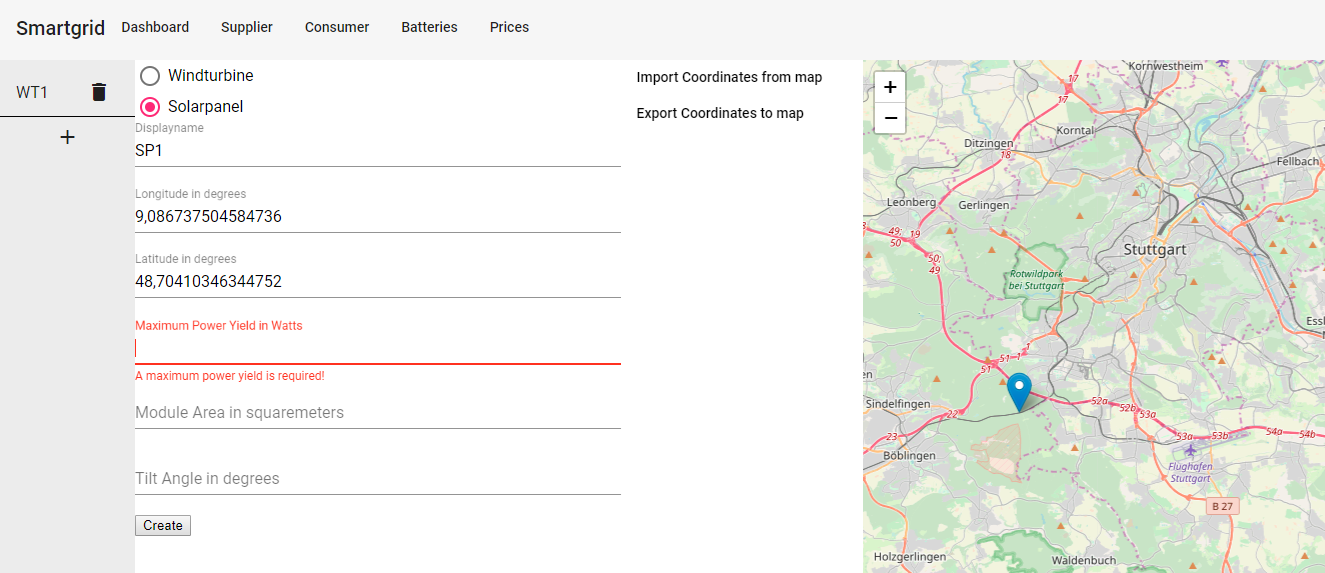
\includegraphics[width=1.00\textwidth]{../figures/supplierView.PNG}
    \caption{View to create, delete or manage suppliers}
    \label{fig:suppliers}
\end{figure}

The interface for suppliers is shown in \cref{fig:suppliers}.
On the left side there is a navigation bar which shows all created supplier.
A user can add a new one using the \textit{plus} button under the suppliers, delete a specific supplier using the \textit{bin} button right to the supplier or manage the supplier by clicking on it.
The main part of this page is the form with the user given data such as latitude, longitude or additional supplier specific needed data, e.g. rotator radius for wind turbines.
The kind of supplier can be chosen with the radio button above the form.
Due to Angulars modularity, it is easy to add more kinds of supplier in the future.
Next to the form is a map using the Angular Leaflet\footnote{\url{https://leafletjs.com/}} openstreetmap API.
The nice part is that a user does not need to know the specific latitude or longitude to create supplier.
Clicking on the map adds a location point which can be exported easily to the form which allows the user to create suppliers at a specific place in the map. To support the user even more, required fields which are left blank are highlighted. This is shown in \cref{fig:suppliers} for the maximal power yield.
Once created a supplier, it is available in the navigation bar at the right.
Clicking on it shows all data already filled in the form and allows the user to change it conveniently. 


\subsection{Batteries}
The batteries view is shown in \cref{fig:batteries}.
It shares a lot of the functionality with the suppliers view to provide a consistent user experience. On the left side of the page, there is the same kind of navigation bar we also used in the supplier and consumer pages to create, delete and manage batteries.
In the middle of the view, there is also a form to set the batteries data.
The user can specify battery capacity, charge, discharge rates and efficiency as well as it's position.
The position can either set directly through the form or just like in the supplier or consumer view through the map using the export button. After pressing the create button the view automatically updates to reflect the changes and to provide the user with feedback for his action. This is also true for suppliers and consumers.

\begin{figure}[!h]
    \centering
    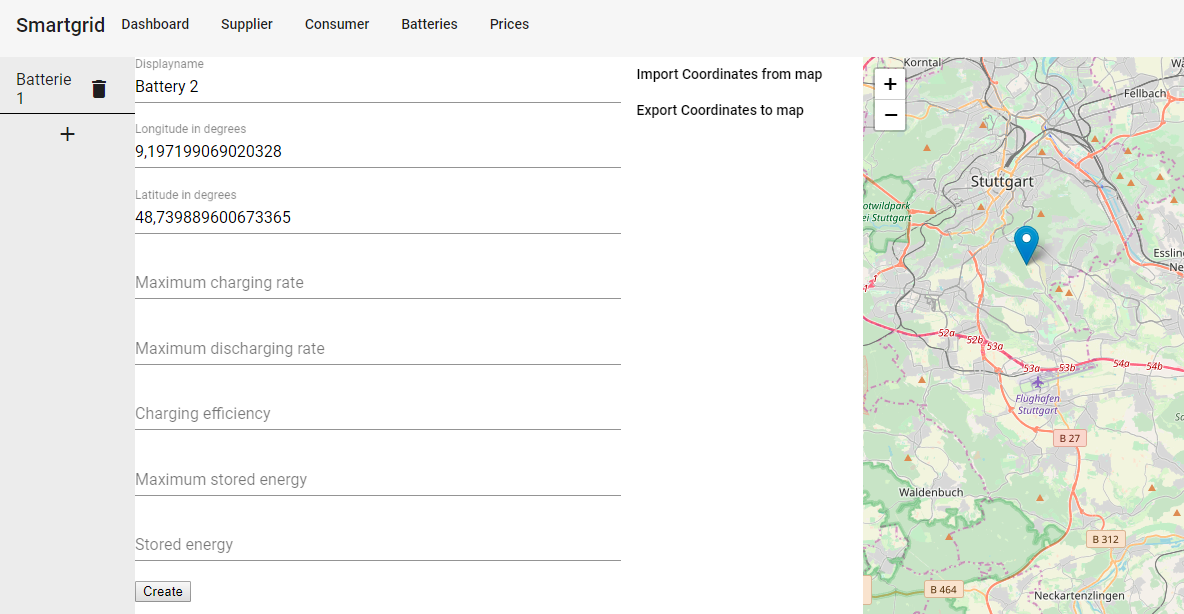
\includegraphics[width=1.00\textwidth]{../figures/batteriesView.PNG}
    \caption{View to create, delete or manage batteries}
    \label{fig:batteries}
\end{figure}


\subsection{Prices}
The prices view shows the energy prices for a preconfigured bidding zone as table and bar chart. The prices originate form ENTSO-E.
The user can specify the start and end date of the prices request, so he can take a look at the day-ahead prices as well as the past 5 days of the energy prices. This process is supported by a date and time picker component to allow a comfortable user experience. 
The page is shown in \cref{fig:prices}. 

\begin{figure}[!h]
    \centering
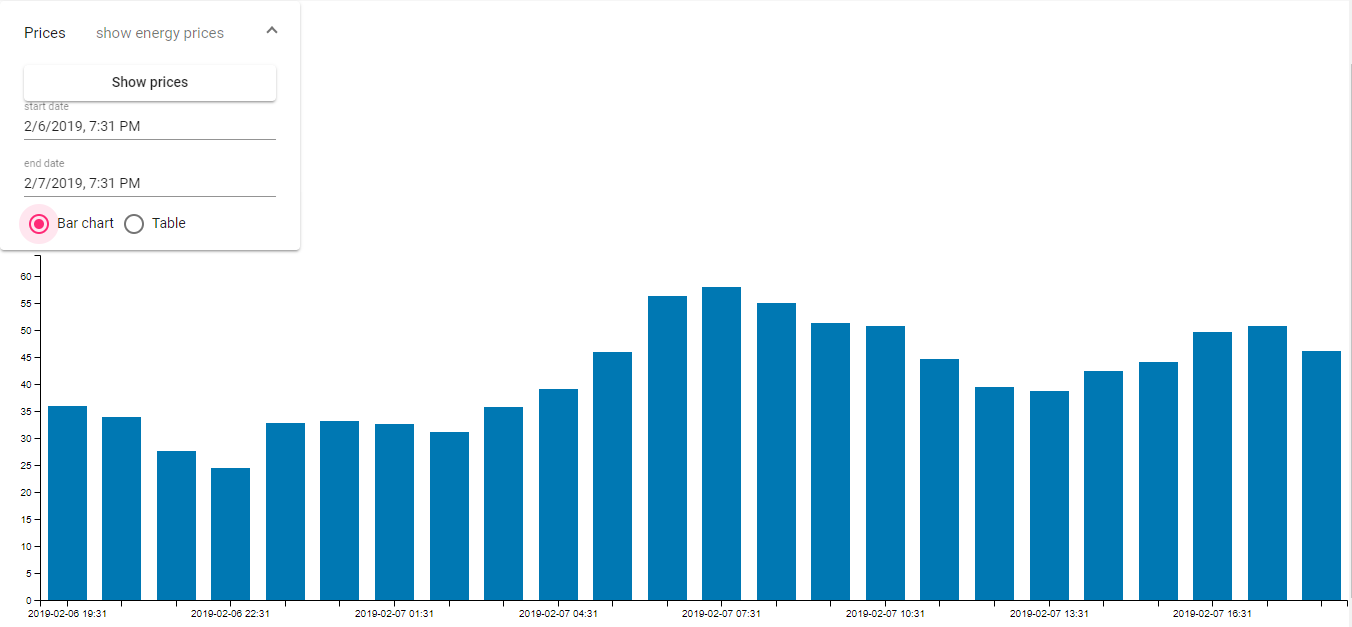
\includegraphics[width=1.00\textwidth]{../figures/prices.PNG}
    \caption{View show energy prices for specific time interval}
    \label{fig:prices}
\end{figure}

\subsection{Dashboard}
The most interesting view is the dashboard.
In this view, the user can take a look easily at different kinds of information in a compact manner.
The view shows supply, demand and other information in a chart, as shown in \cref{fig:dashboard}
Clicking on the labels in the legend (right part of the chart) allows the user to disable or enable data in the chart.
This makes the chart more clear and allows the user to concentrate better on the information he is interested in.
\Cref{fig:consumerChart} shows a chart containing only the consumers.
\begin{figure}[!h]
	\centering
	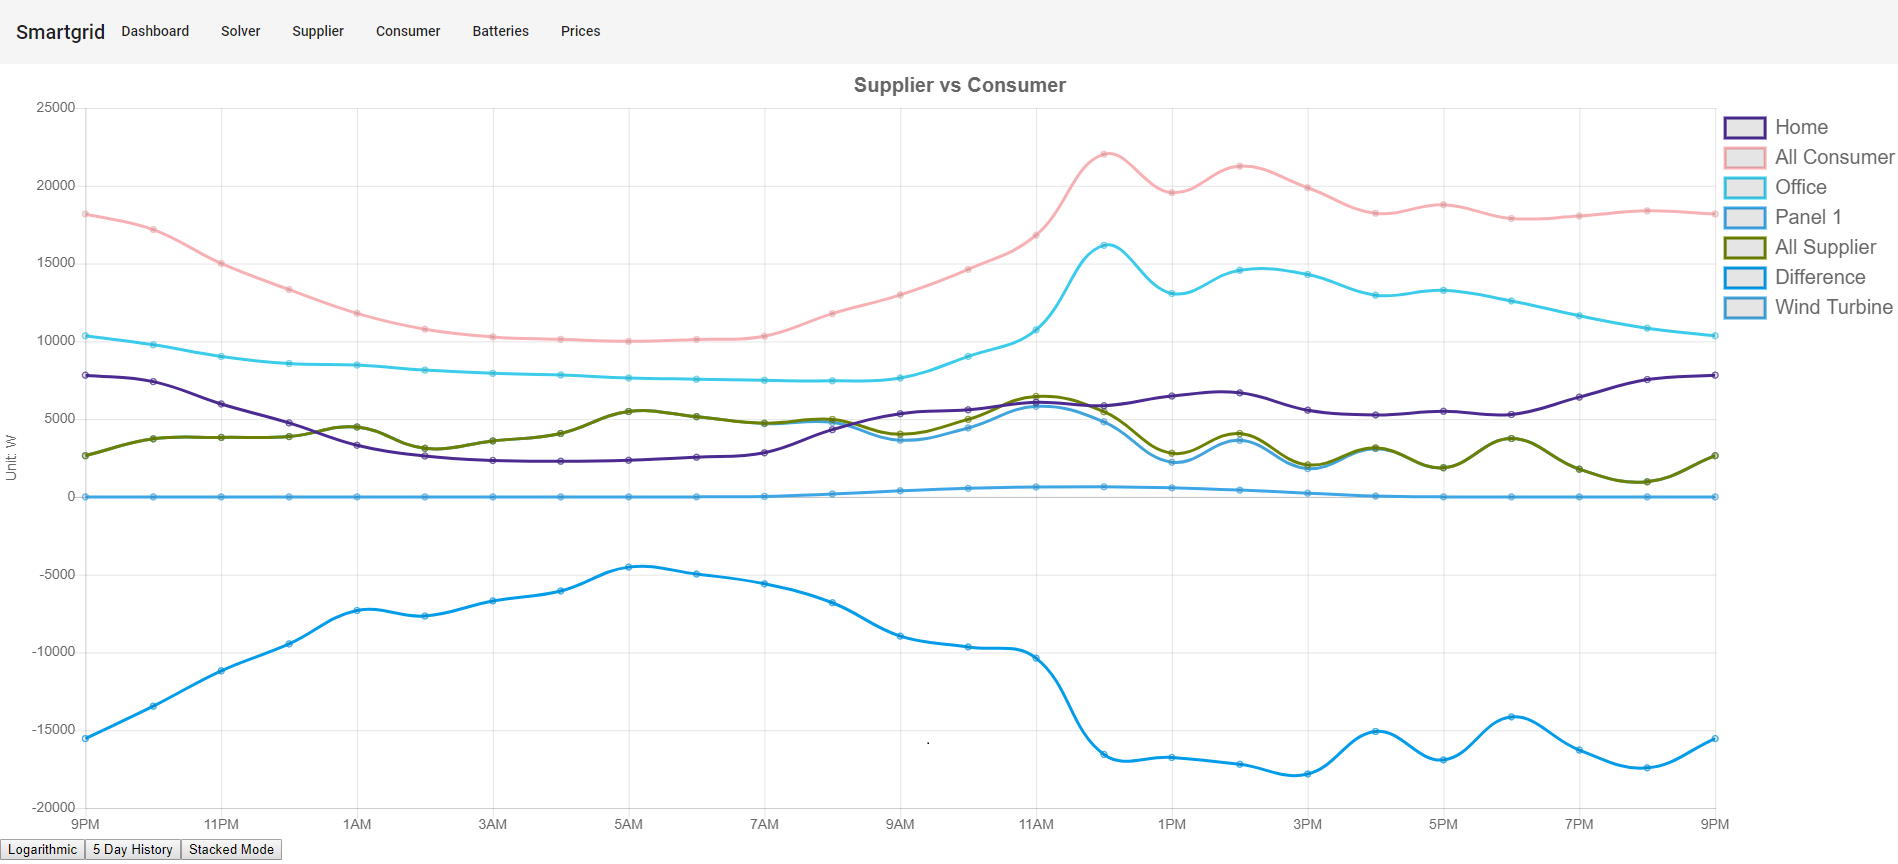
\includegraphics[width=1.00\textwidth]{../figures/OverviewCut.png}
	\caption{Dashboard view to show the charts}
	\label{fig:dashboard}
\end{figure}

\begin{figure}[h]
    \centering
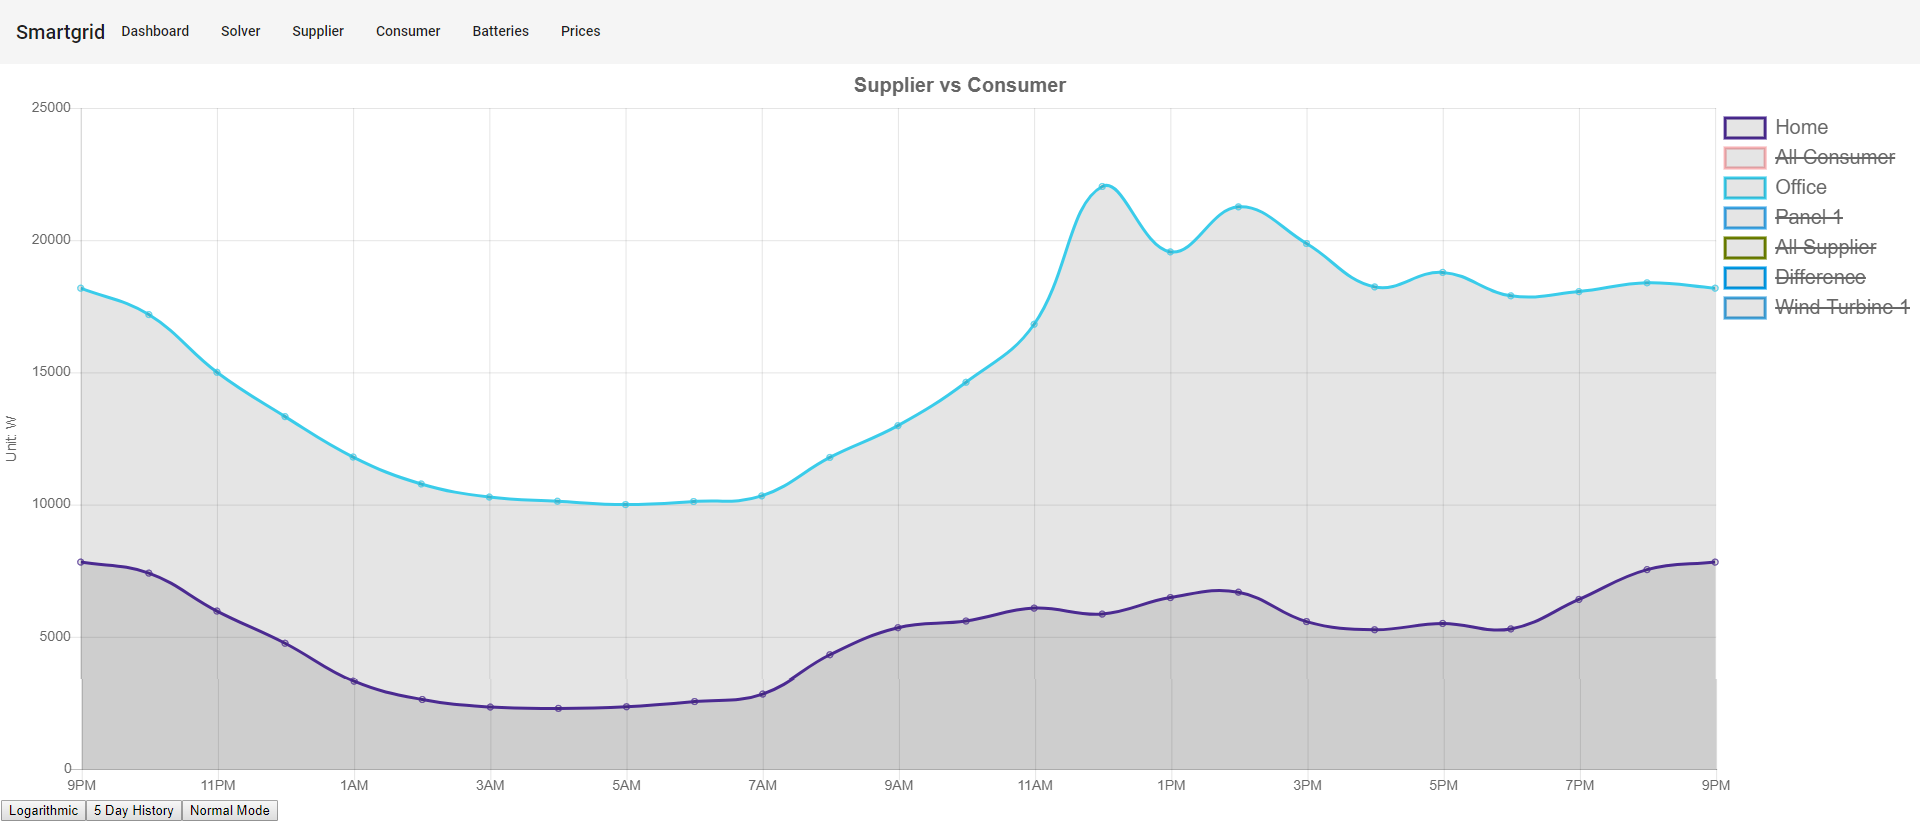
\includegraphics[width=1.00\textwidth]{../figures/ConsumerStackedCut.png}
    \caption{Chart showing only the energy demand of the consumers}
    \label{fig:consumerChart}
\end{figure}

\begin{figure}[!h]
	\centering
	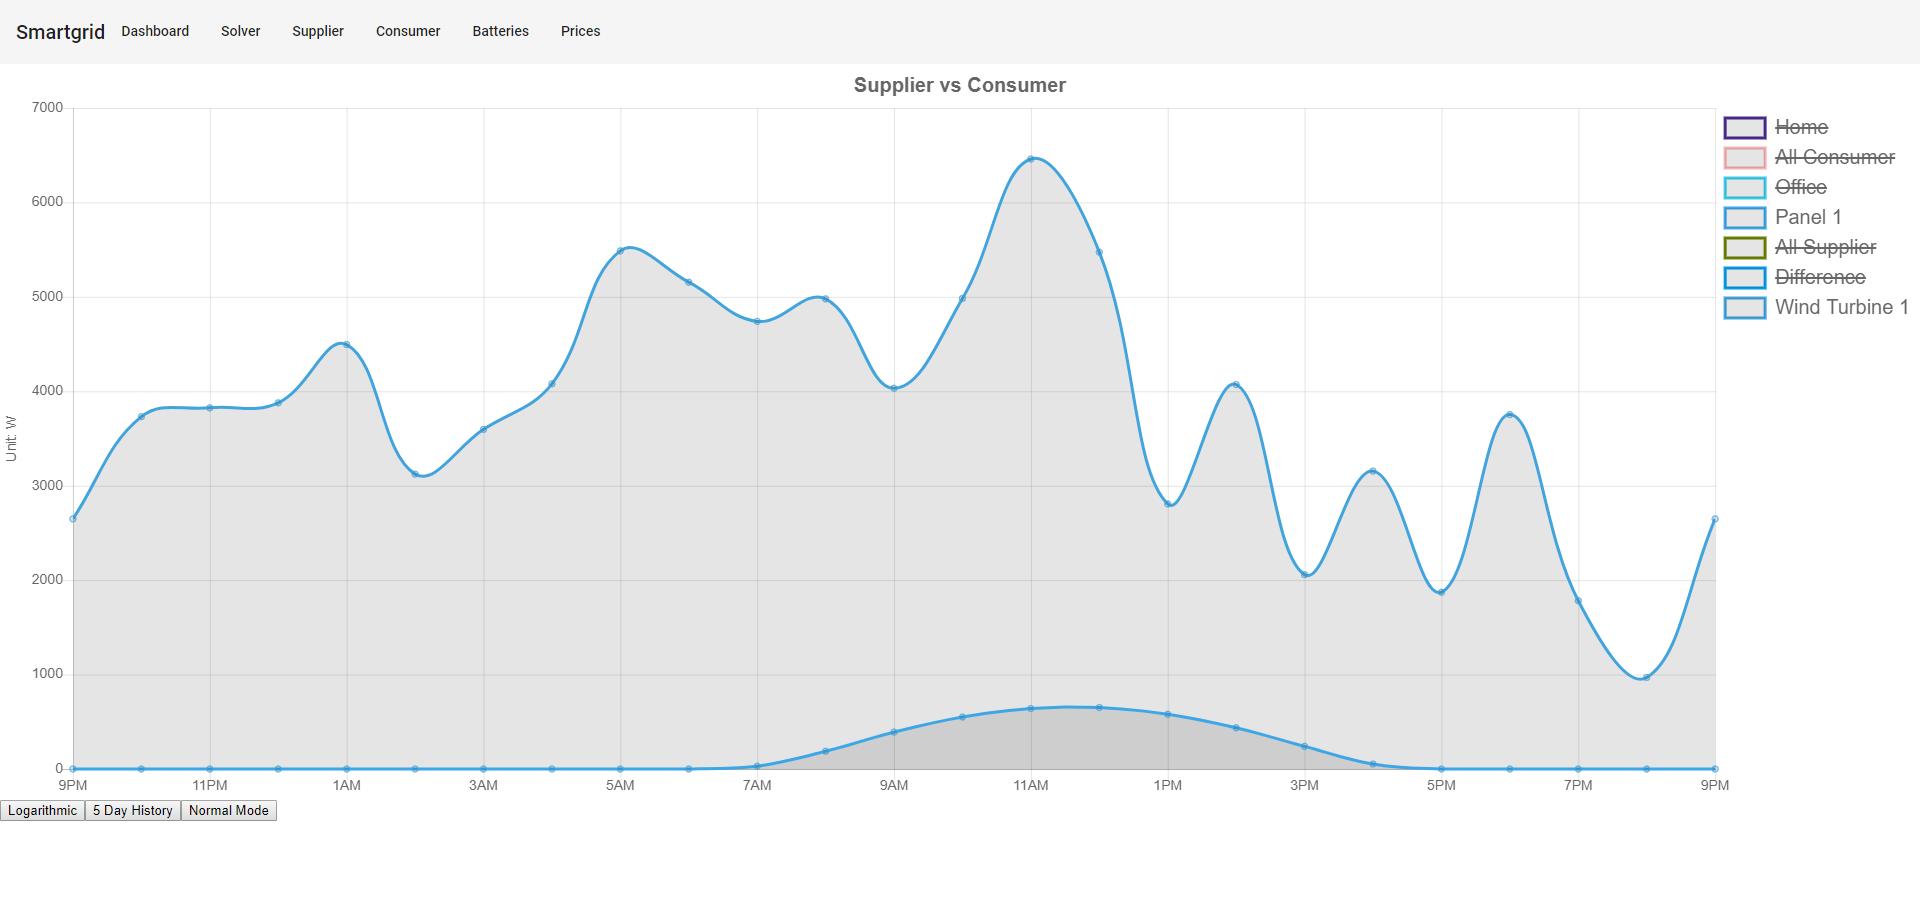
\includegraphics[width=1.00\textwidth]{../figures/SupplierStacked.png}
	\caption{Chart showing only the energy produced by the supplier}
	\label{fig:supplierChart}
\end{figure}

If a user is interested only in the energy produced by the supplier, he can select only the supplier as shown in \cref{fig:supplierChart}.

Using the buttons under the chart switches between several charts.
We provide a logarithmic view or normal view.
In addition to this, we can show the user 5 days history or the forecast.

Sometimes it is useful to see a stacked view of the data. For this reason, we chose to support stacked charts and normal charts.
In stacked charts, the values can be stacked above each others.
In \cref{fig:supplierChart} a stacked chart is used, where the supply of \textit{Panel 1} is added above the supply of \textit{Wind Tubine 1}.
\Cref{fig:dashboard} shows a normal chart.

\subsection{Solver}\label{sec:solver}
\begin{figure}[!h]
    \centering
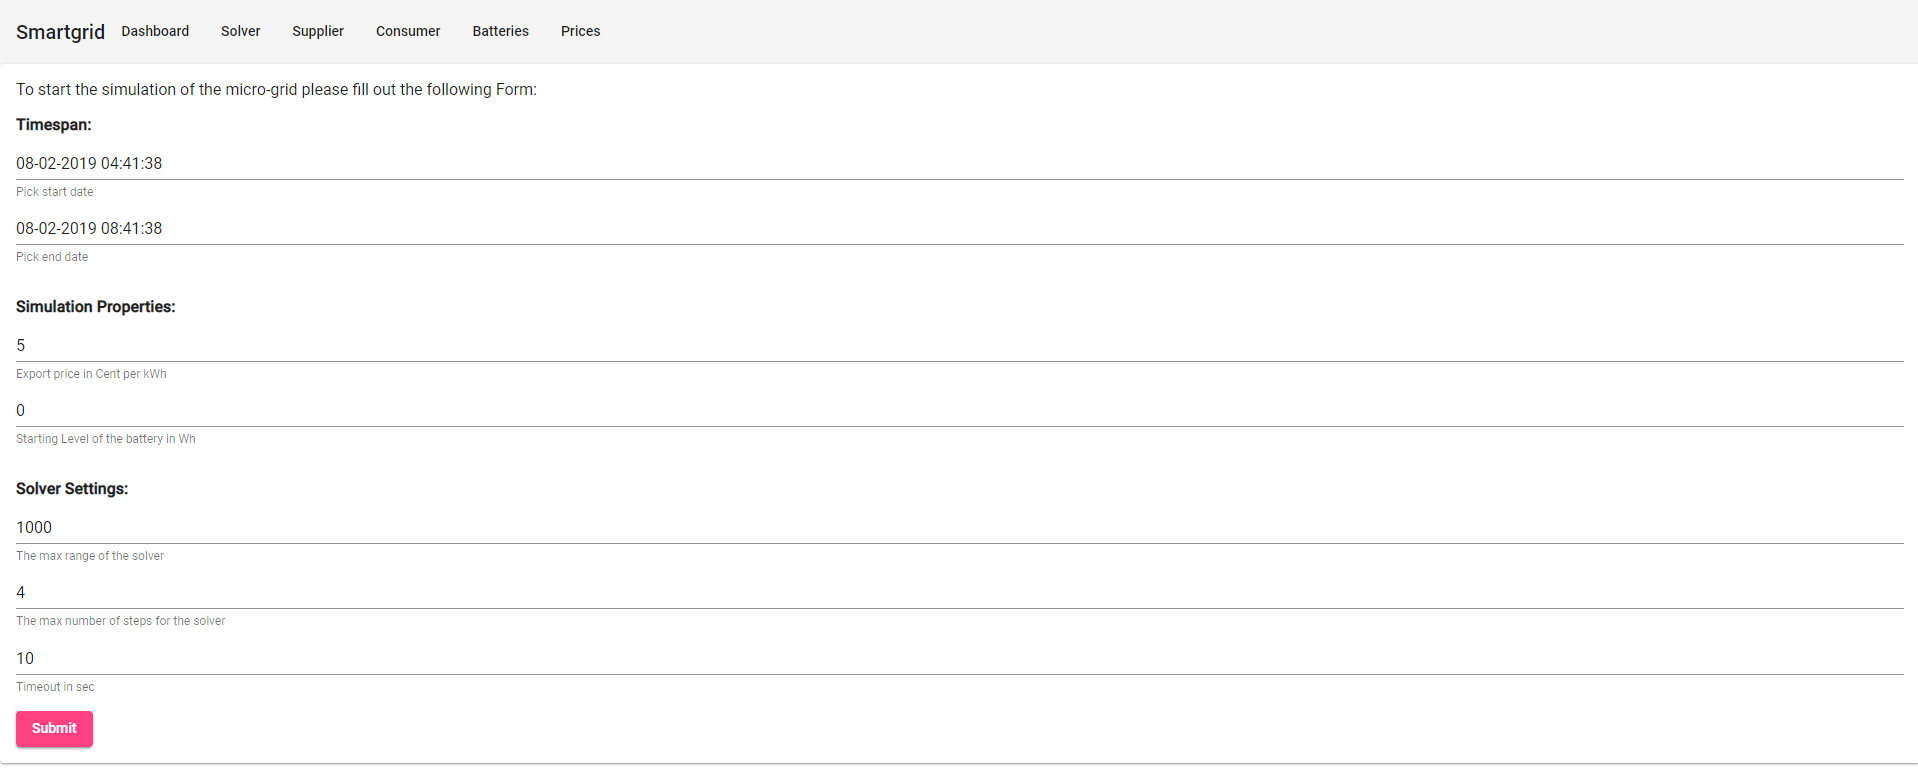
\includegraphics[width=1.00\textwidth]{../figures/SolverSettings2Cut.png}
    \caption{This view is used to configure the solver}
    \label{fig:solverSettings}
\end{figure}
Our system is made to allow a user to simulate a micro-grid for a period of time. 
The user should be able to configure a simulation and then post it to the system. 
After the simulation is complete the results are shown to the user. This could be used to understand the dynamics of a micro-grid. To start a simulation the user has to provide some information.
\Cref{fig:solverSettings} shows the configuration page for a simulation. 
First the user has to enter the start and end time. There is also a date and time picker to ease the user interaction. For the simulation part more information is necessary. Prices for importing energy via the main grid are provided by the price collector. But it is also possible to sell energy. Therefore, the user has to specify the price which he gets for exporting energy to the main grid. It is also possible to start with a filled battery. For this option a fill level can provided. The last group of input information are specific to the solver. To reduce the time which it takes to simulate the micro-grid all values are bound to a range. This range Can be specified but it should be used with caution, because it can increase the run time and the memory consumption enormously. The specific increase depends on the input values and the other settings. The next setting the number of steps which should be calculated. Higher settings increase run time and memory consumption. The last setting is the timeout time. In most instances the solver finds a good or good enough solution quit fast, but it runs for a long time to find a better one. With this setting a user can determine how long the calculation should run before the solver cancels the search end returns the best solution so far. After pressing the Submit button the simulation request is posted to the system and a progress indicator is shown until the results are back. In the result view the user can see the steps of the solver in three possible ways.
The first way is to show the steps in a chart. \Cref{fig:solverChats} contains this chart view. Depending on the values in the chart, it is sometimes hard to overview everything fast. But it is possible to remove information from each chart to improve the readability. But some information and connections are easy to spot, for example that the export profit raises (Chart 2) while the supply also increases. All suppliers and all consumers of one type are aggregated before simulation happens. For instance all suppliers and all homes are combined. This helps to keep the simulation times and the memory consumption at a feasible level. The other view (\cref{fig:solverTable}) is a tabular view which is best to overview all information fast.
There is also the possibility to show a textual description of the steps. The last possibility to view the data is in a very short textual summary for each step.
Under the table, chart or text there is always a summary of the costs and profit of the system.
Each view in this project is designed to help the user and to make interaction as easy as possible while providing a wide selection of possibilities.
\begin{figure}[!h]
	\centering
	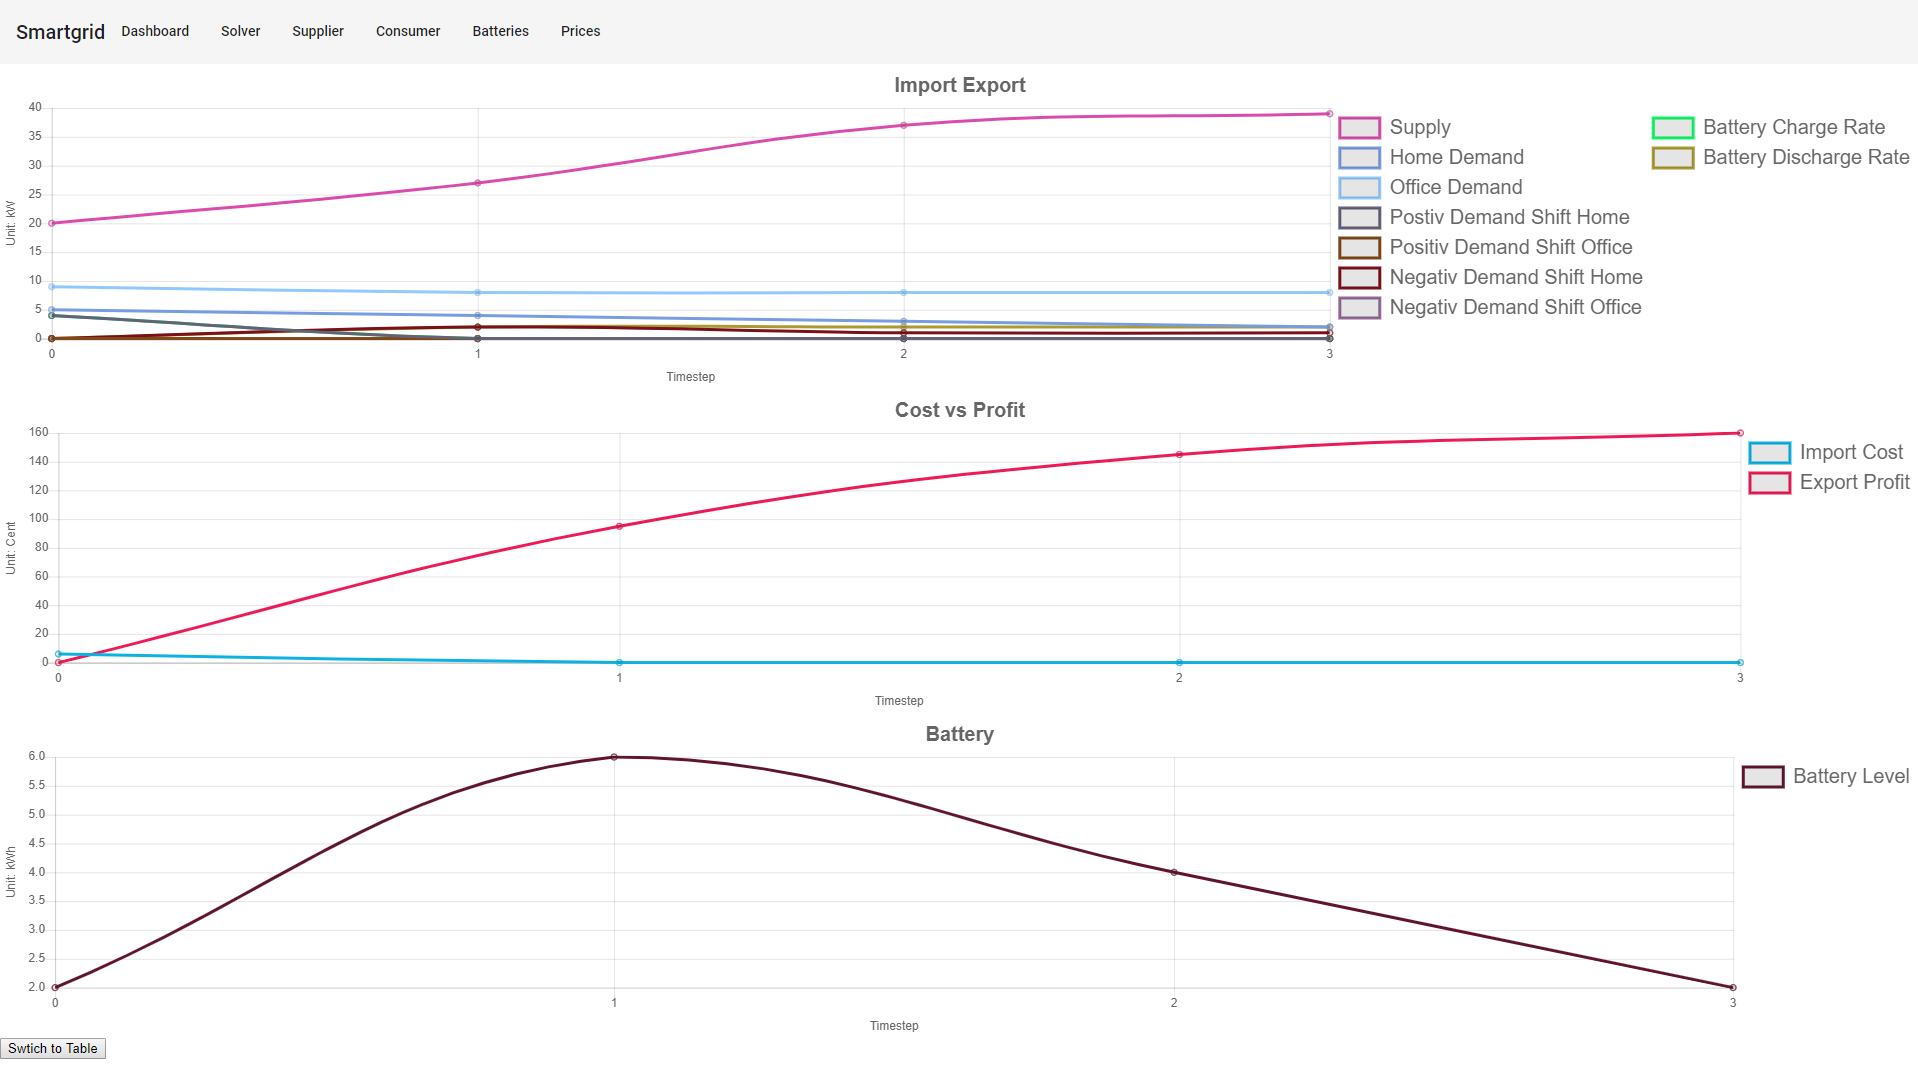
\includegraphics[width=1.00\textwidth]{../figures/SolverChartsCut.png}
	\caption{Chart view of solver steps}
	\label{fig:solverChats}
\end{figure}

\begin{figure}[!h]
    \centering
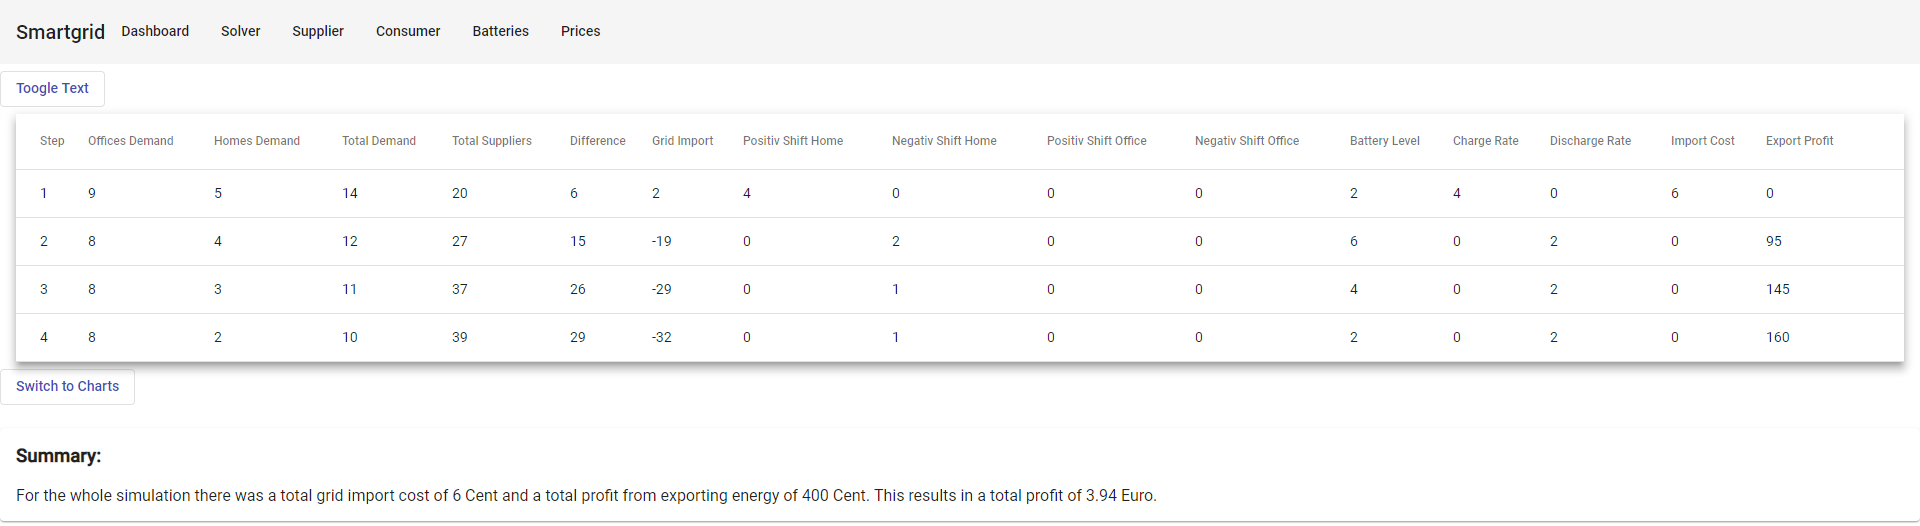
\includegraphics[width=1.00\textwidth]{../figures/SolverTableCut.png}
    \caption{Table view of solver steps}
    \label{fig:solverTable}
\end{figure}